\label{experiments}
\section{Experiments}

In this section, we present the performance comparison of various backpressure variants on our simulator and provide a brief overview of the real-world implementation. All experiments are carried out on a 12 core Intel Xeon CPU E5-1650 machine with 32GB RAM operating at 3.20GHz. We tested a variety of networks with two main traffic matrices - all-to-all traffic matrix and random permutation traffic matrix. All presented results are for n-dimensional hypercubes with all-to-all traffic matrix.

\subsection{Simulations}

\textbf{Basic backpressure algorithm}
\begin{figure}
%\centering
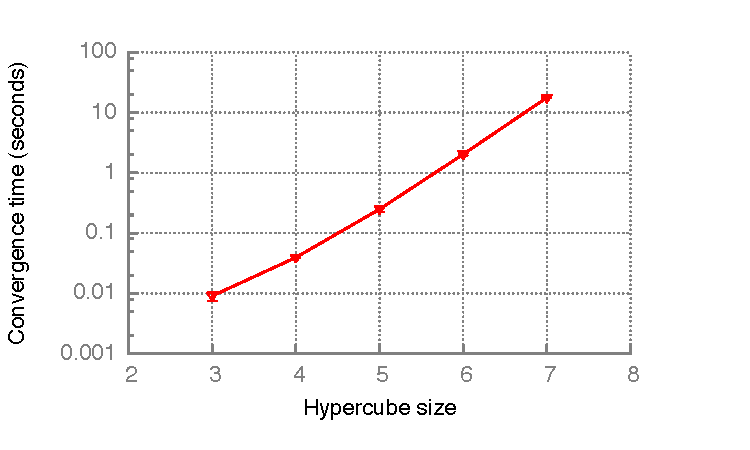
\includegraphics[width=3in, height=2in]{./figures/basic.pdf}
\caption{\small Performance of basic backpressure algorithm}
\label{fig:M_1}
\end{figure}

\textbf{Variation with epsilon}

\textbf{Variation with threshold}
In figure~\ref{fig:M_1},we observe that 
\begin{figure}
%\centering
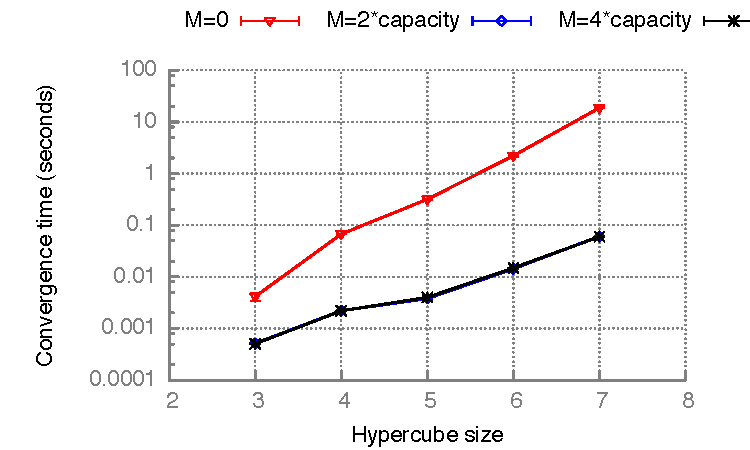
\includegraphics[width=3in, height=2in]{./figures/M_variation.pdf}
\caption{\small Variation of convergence time with M}
\label{fig:M_1}
\end{figure}


\subsection{Real implementation}

